\documentclass{../khlslides}


\title[Algo1]{Introductie}
\author{Fr\'ed\'eric Vogels}

\newcommand{\jscodeblock}[3][]{\begin{block}{#3}\lstinputlisting[language=javascript,#1]{#2}\end{block}}
\newcommand{\X}[2]{\tikz[baseline,remember picture]{\node[anchor=base,inner sep=0mm] (#2) {{#1}};}}


% Segmented pie chart
% \pgfkeys{/mylib/segpie/.cd,
%          fill/.store in=\fill,
%          inner radius/.store in=\innerradius,
%          outer radius/.store in=\outerradius}

\pgfkeys{/mylib/segpie/.cd,
         fill/.initial=white,
         inner radius/.initial=0,
         outer radius/.initial=1
       }

\newcommand{\segpie}[4][]{
  {
    \newcommand{\segment}[3][]{
      {
        \pgfkeys{/mylib/segpie/inner radius/.get=\innerradius}
        \pgfkeys{/mylib/segpie/outer radius/.get=\outerradius}
        \pgfkeys{/mylib/segpie/fill/.get=\fill}
        \pgfmathparse{##2/##3*360}\let\fromangle\pgfmathresult
        \pgfmathparse{(##2+1)/##3*360}\let\toangle\pgfmathresult
        \draw[thin,fill=\fill] (\fromangle:\innerradius) --
                               (\fromangle:\outerradius) --
                               (\toangle:\outerradius) --
                               (\toangle:\innerradius) --
                               cycle;
      }
    }
    \pgfkeys{/mylib/segpie/.cd,#1}
    \foreach \idx in {#2,...,#3} {\segment{\idx}{#4}};
  }
}



\begin{document}

\maketitle

\section{Introductie}

\frame{ \tableofcontents[currentsection] }

\begin{frame}
  \frametitle{Studiebelasting}
  \begin{columns}
    \column{.5\textwidth}
    \begin{center}
      \begin{tikzpicture}
        \pgfkeys{/mylib/segpie/.cd, inner radius=1.5, outer radius=2.5}
        \only<1>{
          \segpie[fill=white]{0}{74}{74}
        }
        \only<2>{
          \segpie[fill=red]{0}{11}{74}
          \segpie[fill=white]{12}{74}{74}
        }
        \only<3>{
          \segpie[fill=red]{0}{11}{74}
          \segpie[fill=blue]{12}{29}{74}
          \segpie[fill=white]{30}{74}{74}
        }
        \only<4>{
          \segpie[fill=red]{0}{11}{74}
          \segpie[fill=blue]{12}{29}{74}
          \segpie[fill=green]{30}{74}{74}          
        }
      \end{tikzpicture}
    \end{center}
    \column{.5\textwidth}
      \begin{itemize}
        \item<1-> 3 studiepunten
        \item<1-> 25 uur per studiepunt
        \item<1-> 12 weken
        \item<1-> $\Rightarrow$ 75 uren in totaal
        \item<1-> $\Rightarrow$ 6.25 uur/week
        \item<2-> {\color{red} 1 uur/week theorie}
        \item<3-> {\color{blue} 1.5 uur/week oefeningen}
        \item<4-> {\color{green} 3.75 uur/week zelfstudie}
      \end{itemize}
  \end{columns}
\end{frame}

\begin{frame}
  \frametitle{Puntenverdeling}
  \begin{columns}
    \column{.5\textwidth}
    \begin{itemize}
      \item {\color{red} 40\%: opdrachten}
             \begin{itemize}
               \item {\color{red} Toetsen}
             \end{itemize}
             \vskip4mm
      \item {\color{blue} 60\%: examen}
             \begin{itemize}
               \item {\color{blue} 10\% mondeling contactexamen}
               \item {\color{blue} 50\% schriftelijk contactexamen}
             \end{itemize}
    \end{itemize}
    \column{.5\textwidth}
    \begin{center}
      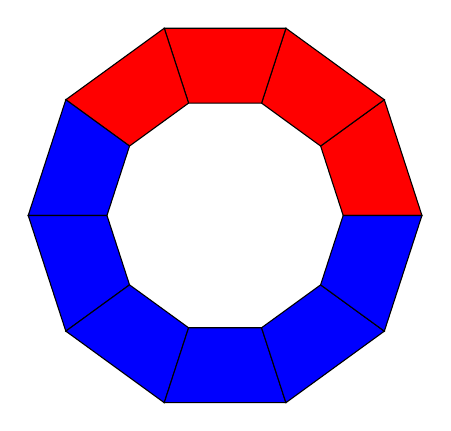
\begin{tikzpicture}
        \pgfkeys{/mylib/segpie/.cd, inner radius=1.5, outer radius=2.5}
        \segpie[fill=red]{0}{3}{10}
        \segpie[fill=blue]{4}{9}{10}
      \end{tikzpicture}
    \end{center}
  \end{columns}
  \vskip5mm
  {\tiny (Offici\"ele informatie te vinden op studiewijzer)}
\end{frame}

\begin{frame}
  \frametitle{Plaatsing}
  \begin{center}
    \begin{tikzpicture}[vak/.style={rectangle,draw=black,fill=blue!25,thin,minimum size=12mm},
                        arr/.style={->,thick},
                        sem/.style={left color=blue!75, right color=blue!25,drop shadow},
                        semc/.style={rotate=90,fill=blue!75,rectangle,drop shadow},
                        lang/.style={circle,fill=red!50,circular drop shadow},
                        langarr/.style={ultra thick,->,red!50}]
      \path[use as bounding box] (-3,0) rectangle (3,5);
      \node[semc] at (-2.25,3.75) {S1};
      \node[semc] at (-2.25,1.75) {S2};
      \node[semc] at (-2.25,-0.25) {S3};
      \shade[sem] (-2,4.75) rectangle (2, 3.25);
      \shade[sem] (-2,2.75) rectangle (2, 1.25);
      \shade[sem] (-2,0.75) rectangle (2, -0.75);
      \node[vak] (bop)    at (-1,4)   {BOP};
      \node[vak] (algo1)  at (1,4)    {Algo1};
      \node[vak] (oop)    at (-1,2)   {OOP};
      \node[vak] (algo2)  at (1,2)    {Algo2};
      \node[vak] (ooo)    at (-1,0)   {OOO};
      \draw[arr] (algo1) -- (bop);
      \draw[arr] (bop) -- (oop);
      \draw[arr] (oop) -- (ooo);
      \draw[arr] (algo1) -- (algo2);
      \draw[arr] (bop) -- (algo2);

      \only<2>{
        \node[lang] (java) at (-4,2.5) {Java};
        \node[lang] (javascript) at (3.75,4) {JavaScript};
        \draw[langarr] (java) to [bend left=45] (bop);
        \draw[langarr] (java) to [bend left=45] (algo2);
        \draw[langarr] (java) to [bend left=45] (oop);
        \draw[langarr] (java) to [bend left=45] (ooo);
        \draw[langarr] (javascript) to [bend right=45] (algo1);
      }
    \end{tikzpicture}
  \end{center}
\end{frame}

\section{Algoritmes}

\frame{ \tableofcontents[currentsection] }

\begin{frame}
  \frametitle{Vierkanswortel}
  \structure{Definitie}
  \[
    y = \sqrt{x} \quad\iff\quad y^2 = x
  \]
  \vskip5mm
  \structure{Voorbeelden}
  \[
    \begin{array}{rcl}
      \sqrt1 & = & 1 \\
      \sqrt4 & = & 2 \\
      \sqrt9 & = & 3 \\
             & \vdots & \\
      \sqrt{100} & = & 10 \\
    \end{array}
  \]
\end{frame}

\begin{frame}
  \frametitle{Vierkantswortel}
  \[
    \sqrt{1000} \quad=\quad ?
  \]
\end{frame}


\begin{frame}
  \frametitle{Vierkantswortel}
  \jscodeblock[basicstyle=\small\tt]{sqrt.js}{Code}
\end{frame}

\begin{frame}
  \frametitle{Algorithms: They're Everywhere}
  \begin{center}
    \begin{tikzpicture}[box/.style={fill=red,opacity=.25,ultra thick},
                        msg/.style={rectangle,fill=red,opacity=.25,text opacity=1}]
      \path[use as bounding box] (-5,-1) rectangle (5,5);
      \node[anchor=south] (pic) at (0,0) { \pgfimage[width=10cm,interpolate=true]{borderlands.jpg} };
      \only<2>{
        \draw[box] (1, 4.5) circle (1);
        \node[msg,anchor=north] at (0, 0) { \parbox{10cm}{ \centering
            Hidden surface removal \\ {\tiny (Z-buffering, Painter's Algorithm, BSP trees, \dots)}
        }};
      }
      \only<3>{
        \draw[box] (-3, 3) circle (1);
        \draw[box] (1.5, 3) circle (.5);
        \node[msg,anchor=north] at (0, 0) { \parbox{10cm}{ \centering
            Hit detection
        }};
      }
      \only<4>{
        \draw[box] (1.85, 2.3) circle (.75);
        \node[msg,anchor=north] at (0, 0) { \parbox{10cm}{ \centering
            Particle system (fire simulation)
        }};
      }
      \only<5>{
        \draw[box] (0, 2) circle (.9);
        \draw[box] (3.5, 1.2) circle (.9);
        \node[msg,anchor=north] at (0, 0) { \parbox{10cm}{ \centering
            Shadow casting (static vs dynamic)
        }};
      }
      \only<6>{
        \draw[box] (0.3, 2.7) circle (.5);
        \node[msg,anchor=north] at (0, 0) { \parbox{10cm}{ \centering
            Artificial Intelligence \\
            {\tiny (Path Finding: A-star, Game Trees: Minimax, Artifical Neural Networks, \dots)}
        }};
      }
    \end{tikzpicture}
  \end{center}
\end{frame}

\begin{frame}
  \frametitle{Algoritmes}
  \begin{itemize}
    \item Stap-voor-stap beschrijving van oplossingsmethode
          \vskip5mm
    \item Drie ``kwaliteitsmetrieken''
          \begin{itemize}
            \item Algoritme moet ooit eindigen
            \item Algoritme moet correct resultaat opleveren
            \item Algoritme moet zo effici\"ent mogelijk werken
          \end{itemize}
          \vskip5mm
    \item Knelpunten
          \begin{itemize}
            \item Enige creativiteit vereist
            \item Randgevallen
            \item Begrijpen van de details
          \end{itemize}
  \end{itemize}
\end{frame}

\begin{frame}
  \frametitle{Puzzel}
  \begin{center}
    \begin{tikzpicture}
      \node { \pgfimage[width=5cm,interpolate=true]{scale.png} };
    \end{tikzpicture}
  \end{center}  
  \begin{overprint}
    \onslide<1>
    \structure{Probleemstelling}
    \begin{itemize}
      \item Gegeven 9 identiek uitziende goudmunten
      \item E\'en ervan is vals, deze is wat lichter
      \item Vind de valse munt met zo weinig mogelijk wegingen
    \end{itemize}

    \onslide<2>
    \structure{Na\"ieve oplossing}
    \begin{itemize}
      \item Telkens twee munten met elkaar vergelijken
      \item Een lichtere gevonden $\rightarrow$ valse munt gevonden
      \item Kan tot 7 wegingen leiden
    \end{itemize}

    \onslide<3>
    \structure{Effici\"entste oplossing}
    \begin{itemize}
      \item Drie munten met drie andere vergelijken
      \item Indien gelijk: valse zit in laatste drie
      \item Anders: kies de lichtste drie
      \item Slechts 2 wegingen nodig
    \end{itemize}

  \end{overprint}
\end{frame}

\begin{frame}
  \frametitle{Overzicht Cursus}
  \begin{enumerate}
    \item Variabelen
    \item Conditionele Logica
    \item Lussen
    \item Functies
    \item Recursie
    \item Rijen
    \item Sorteeralgoritmen
    \item Complexiteit
  \end{enumerate}
\end{frame}

\section{HTML \& JavaScript}

\frame{ \tableofcontents[currentsection] }

\begin{frame}
  \frametitle{HTML}
  \begin{itemize}
    \item HyperText Markup Language
          \vskip4mm
    \item Taal van het world wide web
          \vskip4mm
    \item Gebruikt om webpagina's te defini\"eren
          \vskip4mm
    \item Vergelijkbaar met een Word-document
          \vskip4mm
    \item Voorbeeld: {\tt example.html}
          \vskip4mm
    \item Statisch (onveranderlijk, geen interactie mogelijk)
  \end{itemize}
\end{frame}

\begin{frame}
  \frametitle{JavaScript}
  \begin{itemize}
    \item Geen relatie met Java
          \vskip4mm
    \item Enkel gelijkaardige syntax
          \vskip4mm
    \item Laat toe een HTML document te manipuleren
          \vskip4mm
    \item Kan reageren op user input
          \vskip4mm
    \item Zorgt voor interactieve webpagina's
          \vskip4mm
    \item Bv. gmail, boids
  \end{itemize}
\end{frame}

\begin{frame}
  \frametitle{JavaScript}
  \begin{itemize}
    \item JavaScript hoort bij een HTML document
          \vskip4mm
    \item Geen JavaScript zonder HTML {\tiny (white lie)}
          \vskip4mm
    \item Om een JavaScript programma te schrijven
          \begin{itemize}
            \item HTML bestand aanmaken (minimalistisch)
            \item JavaScript code eraan vasthechten
          \end{itemize}
  \end{itemize}
\end{frame}

\begin{frame}
  \frametitle{JavaScript Embedden}
  \jscodeblock{embed.html}{Embedding}
  \begin{itemize}
    \item Slechts \'e\'en bestand nodig
    \item Gekke syntactische beperkingen
    \item Geen good practice
  \end{itemize}
\end{frame}

\begin{frame}
  \frametitle{JavaScript Linken}
  \jscodeblock{linking.html}{Linking}
  \begin{itemize}
    \item Geen syntactische beperkingen
    \item Algemeen aangeraden manier
    \item Editors kunnen hier gemakkelijker mee om
    \item Twee bestanden
  \end{itemize}
\end{frame}

\end{document}



%%% Local Variables: 
%%% mode: latex
%%% TeX-master: t
%%% End: 
